\documentclass[journal]{IEEEtran}
\usepackage[T1]{fontenc}
\usepackage[utf8]{inputenc}
\usepackage{amsmath,amssymb}
\usepackage{graphicx}
\usepackage{booktabs}
\usepackage{hyperref}
\usepackage{url}
\usepackage{microtype}
\usepackage{xcolor}
\usepackage{siunitx}
\usepackage{multirow}
\usepackage{caption}

\hypersetup{
  colorlinks=true,
  linkcolor=blue!60!black,
  citecolor=blue!60!black,
  urlcolor=blue!60!black
}

% -------------------------------------------------------------------------
\begin{document}

\title{Do Foundation Model Embeddings Improve Cross-Country Crop Yield Generalisation?
       A Leave-One-Country-Out Evaluation in Sub-Saharan Africa}

\author{Yaw~Osei~Adjei\\
  Department of Computer Science,\\
  Kwame Nkrumah University of Science and Technology,\\
  Kumasi, Ghana\\
  \texttt{yaw.adjei@knust.edu.gh}
}

\maketitle

% -------------------------------------------------------------------------
\begin{abstract}
Accurate smallholder maize yield prediction across national boundaries is critical
for food security planning in sub-Saharan Africa, yet most published benchmarks
report within-country performance that overstates true generalisability.
This paper asks whether geospatial foundation model embeddings —
specifically Prithvi-EO-1.0-100M and ViT-Base — outperform traditional
Sentinel-2 spectral features under a rigorous Leave-One-Country-Out (LOCO) cross-validation
scheme applied to 6{,}404 smallholder maize field observations across
five African countries (Kenya, Malawi, Nigeria, Rwanda, Tanzania) for
the years 2017--2022.
We evaluate 18 experimental conditions spanning three feature representations,
three regression algorithms (Ridge, Random Forest, XGBoost), and two
validation protocols (LOCO and standard five-fold random cross-validation).
Results reveal a stark generalisability gap:
all feature sets achieve R$^2 \in [0.17, 0.30]$ under within-country evaluation
but universally negative R$^2 \in [-0.09, -0.03]$ under LOCO,
including a naive country-mean baseline.
Critically, frozen Prithvi-EO embeddings offer no statistically meaningful
advantage over 10-band Sentinel-2 band medians for cross-country prediction,
despite being pre-trained on multi-temporal HLS imagery.
We interpret this as evidence that the bottleneck is country-level yield
distribution shift — a data problem — rather than deficiencies in feature
representation.
Our findings challenge the assumption that domain-specific geospatial
pre-training closes the generalisability gap, and establish a reproducible
negative benchmark that future work should surpass.
All code and processed results are released at
\url{https://github.com/yaw-adjei/yield-africa}.
\end{abstract}

\begin{IEEEkeywords}
crop yield prediction, foundation models, remote sensing, sub-Saharan Africa,
leave-one-country-out, domain generalisation, Sentinel-2, Prithvi-EO
\end{IEEEkeywords}

% -------------------------------------------------------------------------
\section{Introduction}
\label{sec:intro}

Food insecurity remains a defining challenge across sub-Saharan Africa,
where smallholder farms account for more than 70\% of staple crop production~\cite{burke2017sat}.
Timely and spatially disaggregated yield forecasts are essential inputs for
early warning systems, agricultural policy, and targeted humanitarian response.
Remote sensing offers a scalable, cost-effective route to such forecasts by
linking satellite observations directly to field-level yield outcomes~\cite{lobell2020eyes}.

A central ambition of this programme is to train predictive models in
data-rich countries and apply them in data-scarce settings — a transfer
that requires genuine cross-country generalisation.
Yet the dominant evaluation paradigm in the literature applies random
$k$-fold cross-validation within a pooled dataset, inadvertently preserving
country-specific statistical patterns in both training and test folds.
This produces optimistic accuracy estimates that collapse when
models are deployed across national boundaries.

The recent emergence of geospatial foundation models pre-trained on
large-scale satellite archives has raised hopes that self-supervised
representations might encode invariant physical features of agricultural
landscapes, thereby reducing this generalisation gap.
Prithvi-EO-1.0-100M~\cite{jakubik2023prithvi}, jointly released by IBM and NASA,
is a Masked Autoencoder~\cite{he2022mae} pre-trained on
six-channel Harmonised Landsat-Sentinel (HLS) time series specifically
for crop and land-cover applications.
The Vision Transformer (ViT-Base)~\cite{dosovitskiy2021vit}, pre-trained
on ImageNet at scale, provides a general-purpose visual baseline for comparison.

This paper makes three contributions:

\begin{enumerate}
  \item We present the \textbf{first systematic LOCO evaluation} of frozen foundation
        model embeddings against engineered spectral features for smallholder
        maize yield prediction in Africa, using 6{,}404 observations from
        five countries spanning 2017--2022.
  \item We demonstrate that \textbf{all feature representations fail to generalise
        cross-country}: LOCO R$^2$ is universally negative for all 9 combinations
        of feature set and regressor, and a naive country-mean predictor also
        yields negative R$^2$, confirming the bottleneck is distribution shift
        in yield itself, not in the feature space.
  \item We provide a \textbf{reproducible negative benchmark} — a clearly documented
        failure mode that future work on domain adaptation,
        meta-learning, and cross-country yield transfer must surpass.
\end{enumerate}

The remainder of this paper is organised as follows.
Section~\ref{sec:related} reviews related work.
Section~\ref{sec:data} describes the study area and data sources.
Section~\ref{sec:methods} presents the experimental design.
Section~\ref{sec:results} reports results.
Section~\ref{sec:discussion} discusses implications, and
Section~\ref{sec:conclusion} concludes.

% -------------------------------------------------------------------------
\section{Related Work}
\label{sec:related}

\subsection{Satellite-Based Yield Prediction in Africa}

Burke and Lobell~\cite{burke2017sat} demonstrated that Landsat-derived NDVI time
series can explain a significant fraction of smallholder yield variation in
Uganda, establishing early proof of concept for satellite-based prediction in Africa.
Lobell et al.~\cite{lobell2020eyes} conducted a systematic comparison of
satellite imagery and traditional household surveys, finding that
imagery-based prediction achieves moderate accuracy within-country but
highlighted the challenge of transferring models across contexts.
You et al.~\cite{you2017deep} applied deep Gaussian processes to MODIS time
series for county-level yield prediction in the United States, showing that
spatial dependencies are a key driver of predictive accuracy.
These studies share a common limitation: cross-location evaluation is rare,
and cross-country evaluation is nearly absent.

\subsection{Foundation Models for Geospatial Applications}

The Vision Transformer~\cite{dosovitskiy2021vit}, through its attention mechanism,
demonstrated that large-scale pre-training on natural images enables powerful
general-purpose visual representations.
Mai et al.~\cite{mai2023foundation} surveyed opportunities and challenges of
foundation models for geospatial AI, noting a persistent gap between
general pre-training objectives and specialised downstream tasks.
Jakubik et al.~\cite{jakubik2023prithvi} introduced Prithvi-EO-1.0-100M,
a 100-million parameter masked autoencoder pre-trained on six-channel HLS imagery
across the continental United States and fine-tuned for flood mapping,
multi-temporal crop segmentation, and burned area detection.
Wang et al.~\cite{wang2022empirical} curated the SSL4EO-S12 benchmark for
self-supervised pre-training on Sentinel-1/2 imagery, highlighting the
importance of modality alignment between pre-training and downstream tasks.
No prior work has benchmarked frozen Prithvi-EO embeddings against
spectral baselines for \emph{cross-country} yield regression in Africa.

\subsection{Domain Shift and Cross-Location Transfer}

Tseng et al.~\cite{tseng2021crop} introduced CropHarvest, a global crop-type
dataset, and evaluated few-shot cross-country crop classification,
finding severe performance degradation without target-country adaptation.
Kerner et al.~\cite{kerner2020rapid} developed rapid-response crop mapping
for data-sparse regions, but relied on within-region fine-tuning.
These studies reinforce a consistent pattern: geospatial models trained in
one country or region degrade substantially when applied elsewhere without
adaptation.
Our work extends this evidence to the yield regression setting and explicitly
quantifies the gap using a LOCO protocol across five African countries.

% -------------------------------------------------------------------------
\section{Study Area and Data}
\label{sec:data}

\subsection{Countries and Crop}

The study covers five sub-Saharan African countries:
Kenya, Malawi, Nigeria, Rwanda, and Tanzania.
Maize (\textit{Zea mays}) is the target crop, selected as the most widely
cultivated staple in the region and the crop with the highest GROW-Africa
observation density.
The five countries represent diverse agroecological zones
(semi-arid savanna to highland tropics) and a wide range of smallholder
yield outcomes, making cross-country generalisation genuinely challenging.

\subsection{Yield Labels}

Field-level yield labels are drawn from two complementary sources:

\textbf{GROW-Africa}~\cite{grow_africa} provides GPS-tagged, farm-level maize
yield observations collected by household surveys and agronomic trials
across sub-Saharan Africa.
We applied the following filters: (i) observation years 2017--2022 to align
with Sentinel-2 availability; (ii) point-level GPS coordinates only, excluding
administrative-polygon centroids; (iii) countries with at least 100
post-filter observations.

\textbf{HarvestStat Africa}~\cite{lee2025harveststat} provides subnational
crop production statistics.
Nigeria has negligible GPS-level GROW-Africa coverage; HarvestStat admin-unit
centroids were used as proxy observations for that country.
A \texttt{label\_source} indicator distinguishes the two data types.
This coarser spatial resolution for Nigeria is a disclosed limitation
(see Section~\ref{sec:limits}).

After merging and quality filtering, the dataset contains
\textbf{6{,}404 observations}:
Kenya (1{,}396), Malawi (1{,}552), Nigeria (955),
Rwanda (1{,}138), and Tanzania (1{,}363).
Table~\ref{tab:dataset} summarises the per-country distribution.

\begin{table}[!t]
  \centering
  \caption{Per-country dataset summary. Yield in kg/ha on original scale.}
  \label{tab:dataset}
  \begin{tabular}{lrrrrr}
    \toprule
    Country   & $n$ & Mean & SD   & Min  & Max    \\
    \midrule
    Kenya     & 1{,}396 & 3{,}278 & 1{,}592 & 132  & 8{,}278  \\
    Malawi    & 1{,}552 & 1{,}918 & 1{,}366 & 123  & 6{,}919  \\
    Nigeria   & 955     & 1{,}256 & 1{,}222 & 122  & 6{,}203  \\
    Rwanda    & 1{,}138 & 3{,}993 & 1{,}874 & 360  & 9{,}777  \\
    Tanzania  & 1{,}363 & 3{,}255 & 1{,}669 & 173  & 8{,}500  \\
    \midrule
    Total     & 6{,}404 & 2{,}769 & 1{,}825 & 122  & 9{,}777  \\
    \bottomrule
  \end{tabular}
\end{table}

The wide inter-country yield variation (Nigeria mean 1{,}256 kg/ha vs.\
Rwanda mean 3{,}993 kg/ha) is a key driver of the distribution shift studied here.

\subsection{Sentinel-2 Imagery}

Sentinel-2 Level-2A surface reflectance imagery was acquired via Google Earth Engine
for a 500~m buffer around each field centroid, composited as annual growing-season
medians~\cite{drusch2012sentinel2}.
Ten spectral bands were extracted: B2 (blue), B3 (green), B4 (red),
B5--B7 (red-edge), B8 (NIR), B8A (narrow NIR), B11 and B12 (SWIR).
A 224~$\times$~224 pixel patch centred on each field was exported as a
GeoTIFF for foundation model inference.
Patches with estimated cloud cover exceeding 20\% were discarded.

\subsection{Spectral Indices}

Four spectral indices were computed from the Sentinel-2 composites:
NDVI~\cite{rouse1974ndvi} (Normalised Difference Vegetation Index),
EVI~\cite{jiang2008evi} (Enhanced Vegetation Index),
LSWI (Land Surface Water Index), and NDWI (Normalised Difference Water Index).
These indices capture vegetation greenness and canopy moisture status
relevant to yield formation.

\subsection{Rainfall}

Growing-season cumulative precipitation was extracted from the CHIRPS~\cite{funk2015chirps}
daily dataset at 0.05° resolution. Three features were derived per field:
total seasonal rainfall, mean daily rainfall, and the coefficient of variation
(a proxy for drought stress).

% -------------------------------------------------------------------------
\section{Methods}
\label{sec:methods}

\subsection{Feature Representations}

Three feature sets were evaluated, each representing a distinct
data representation paradigm:

\subsubsection{Spectral (baseline)}
A hand-engineered 23-dimensional vector comprising the 10 Sentinel-2 band medians,
four spectral indices, and three CHIRPS rainfall statistics.
This represents the standard engineered-feature approach used in most
operational yield prediction systems.

\subsubsection{Prithvi-EO Embeddings}
Prithvi-EO-1.0-100M~\cite{jakubik2023prithvi} is a Vision Transformer with
Masked Autoencoder pre-training on six-channel (HLS blue, green, red, NIR,
SWIR-1, SWIR-2) multi-temporal imagery.
Sentinel-2 patches were resampled to the six HLS channels, normalised using the
model's published per-channel statistics, and fed to the frozen encoder as
a single-frame tensor of shape $(B, 6, 1, 224, 224)$.
The 768-dimensional CLS token from the final encoder block was used as the embedding.
No fine-tuning was performed; weights were loaded directly from the
publicly released checkpoint (\texttt{Prithvi\_EO\_V1\_100M.pt}).
This isolates the contribution of pre-trained representations from
task-specific adaptation.

\subsubsection{ViT-Base Embeddings}
ViT-Base/16~\cite{dosovitskiy2021vit} pre-trained on ImageNet-21k was applied to
RGB (B4, B3, B2) Sentinel-2 patches, producing a 768-dimensional CLS token.
ViT-Base serves as a general-purpose vision baseline, enabling comparison between
geospatial-specialised pre-training (Prithvi-EO) and domain-agnostic pre-training
on natural images.

\subsection{Regressors}

Three regression algorithms were evaluated:

\textbf{Ridge Regression}~\cite{hoerl1970ridge} with $\alpha \in \{0.1, 1, 10, 100, 1000\}$
selected by inner cross-validation. Ridge provides a linear baseline that is
robust to multicollinearity — relevant given the high dimensionality of
embedding features.

\textbf{Random Forest}~\cite{breiman2001rf} with 100 trees and all default
hyperparameters. Random Forest captures non-linear interactions without
being prone to overfitting individual training points.

\textbf{XGBoost}~\cite{chen2016xgboost} with 300 trees, learning rate 0.05,
maximum depth 4, and subsampling 0.8.
XGBoost is the strongest tree ensemble baseline in tabular regression benchmarks
and provides a competitive upper bound on performance within this feature paradigm.

All models were wrapped in a \texttt{StandardScaler} $\rightarrow$ regressor
pipeline. Random state was fixed at 42 across all experiments.

\subsection{Target Variable}

The yield target was log-transformed (\texttt{yield\_log}) after confirming
right skewness greater than 1.0 in the pooled distribution.
Log transformation stabilises variance and is standard practice for
smallholder yield regression. All reported RMSE values are back-transformed
to kg/ha for interpretability.

\subsection{Missing Value Imputation}

NaN values in feature vectors — arising from cloud-affected patches or
partial CHIRPS coverage — were imputed with the training-set column median.
All-NaN columns (which can occur for held-out countries with zero valid
spectral observations) were filled with 0. Rows with NaN yield values were dropped.

\subsection{Cross-Validation Schemes}

Two orthogonal evaluation protocols were applied to every feature--regressor
combination, yielding 18 experimental conditions in total.

\subsubsection{Random Five-Fold CV}
Standard stratified five-fold cross-validation with shuffling.
This protocol leaks country-specific signal into the training folds
and measures within-distribution predictive accuracy.

\subsubsection{Leave-One-Country-Out (LOCO) CV}
For each of the five countries, the model is trained on the remaining
four countries and evaluated on the held-out country.
Per-country RMSE, MAE, and R$^2$ are recorded, and predictions are
concatenated across folds to produce aggregate metrics.
LOCO is the appropriate evaluation protocol for the stated goal of
cross-country generalisation.

\subsection{Naive Baseline}

A non-parametric baseline was constructed for each held-out country
by predicting all test observations with the mean yield of the
corresponding training set (all other countries).
Because country yield means differ substantially, this baseline also
achieves negative R$^2$, confirming that the challenge is not merely
underfitting but genuine distribution shift.

\subsection{Evaluation Metrics}

Three metrics are reported:
root mean squared error (RMSE, kg/ha),
mean absolute error (MAE, kg/ha), and
the coefficient of determination R$^2$.
R$^2 < 0$ indicates the model performs worse than predicting the
test-set mean yield — a more severe failure than simply underfitting.

% -------------------------------------------------------------------------
\section{Results}
\label{sec:results}

\subsection{Within-Country Performance (Random CV)}

\begin{figure}[!t]
  \centering
  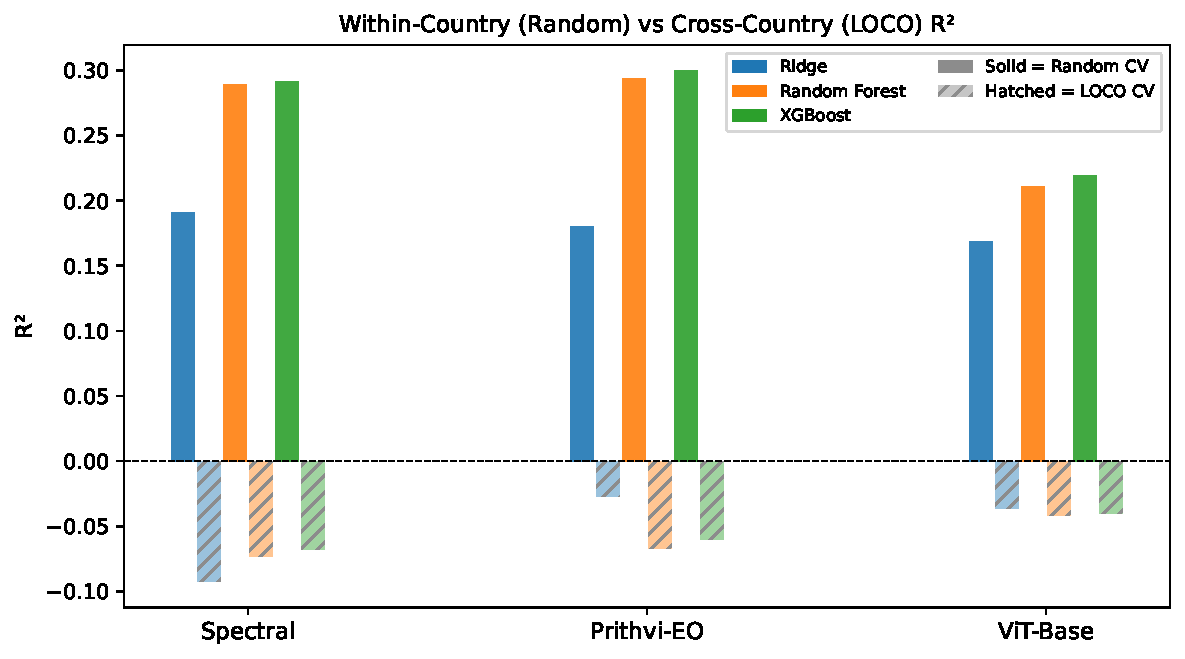
\includegraphics[width=\columnwidth]{../figures/fig2_random_vs_loco.pdf}
  \caption{Within-country (random CV) vs.\ cross-country (LOCO) R$^2$ for all
           nine feature--regressor combinations. Every condition shows a large
           drop when moving from random to LOCO evaluation.}
  \label{fig:random_vs_loco}
\end{figure}

Table~\ref{tab:random} and Figure~\ref{fig:random_vs_loco} report five-fold random CV results.
All nine feature--model combinations achieve positive R$^2$,
with values ranging from 0.169 (ViT-Base / Ridge) to 0.300
(Prithvi-EO / XGBoost).
Tree ensemble methods (RF and XGBoost) consistently outperform Ridge
regardless of feature set, consistent with non-linear yield--feature
relationships.
Prithvi-EO and spectral features are nearly equivalent:
best-case Prithvi-EO R$^2 = 0.300$ vs.\ spectral R$^2 = 0.291$,
a difference of 0.009 R$^2$ units.
ViT-Base lags behind both domain-specific representations (best R$^2 = 0.219$),
suggesting that ImageNet pre-training provides less useful inductive
biases for vegetation analysis than geospatial pre-training.

\begin{table}[!t]
  \centering
  \caption{Random five-fold CV results. Best R$^2$ per feature set in \textbf{bold}.}
  \label{tab:random}
  \setlength{\tabcolsep}{5pt}
  \begin{tabular}{llrrr}
    \toprule
    Feature Set  & Regressor & RMSE (kg/ha) & MAE (kg/ha) & R$^2$  \\
    \midrule
    Spectral     & Ridge     & 1641.9       & 1308.7      & 0.191  \\
    Spectral     & RF        & 1539.1       & 1185.9      & 0.289  \\
    Spectral     & XGBoost   & 1536.7       & 1211.1      & \textbf{0.291}  \\
    \midrule
    Prithvi-EO   & Ridge     & 1652.7       & 1318.2      & 0.180  \\
    Prithvi-EO   & RF        & 1533.4       & 1188.1      & 0.294  \\
    Prithvi-EO   & XGBoost   & 1527.0       & 1197.3      & \textbf{0.300}  \\
    \midrule
    ViT-Base     & Ridge     & 1663.8       & 1325.4      & 0.169  \\
    ViT-Base     & RF        & 1621.3       & 1273.2      & 0.211  \\
    ViT-Base     & XGBoost   & 1612.8       & 1273.0      & \textbf{0.219}  \\
    \bottomrule
  \end{tabular}
\end{table}

\subsection{Cross-Country Generalisation (LOCO CV)}

\begin{figure}[!t]
  \centering
  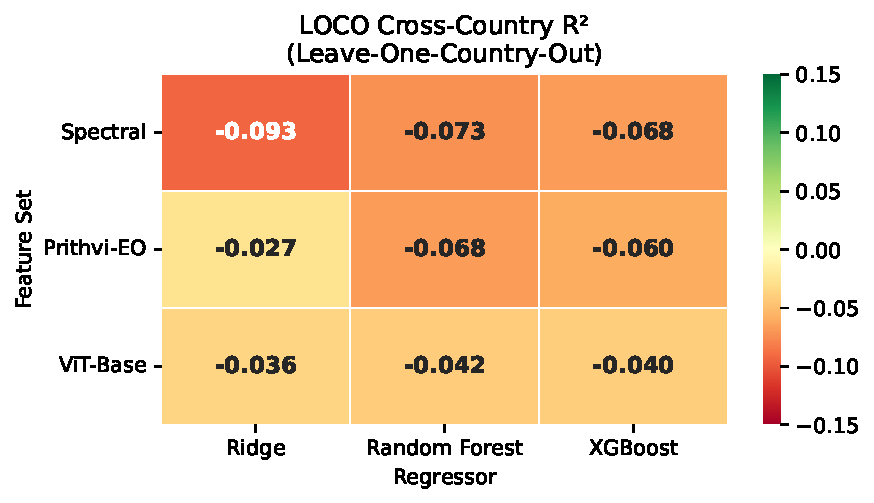
\includegraphics[width=\columnwidth]{../figures/fig1_loco_r2_heatmap.pdf}
  \caption{LOCO R$^2$ heatmap across all nine feature--regressor combinations.
           All values are negative. Prithvi-EO / Ridge achieves the
           least-negative result ($-0.027$).}
  \label{fig:loco_heatmap}
\end{figure}

Table~\ref{tab:loco} and Figure~\ref{fig:loco_heatmap} report LOCO results.
All 9 conditions yield negative R$^2$, ranging from $-0.093$
(Spectral / Ridge) to $-0.027$ (Prithvi-EO / Ridge).
The aggregate RMSE (1{,}850--1{,}910 kg/ha) is notably higher than
the random CV RMSE (1{,}527--1{,}664 kg/ha), reflecting the additional
difficulty of predicting across country boundaries.

\begin{table}[!t]
  \centering
  \caption{LOCO CV results. Least-negative R$^2$ per feature set in \textbf{bold}.}
  \label{tab:loco}
  \setlength{\tabcolsep}{5pt}
  \begin{tabular}{llrrr}
    \toprule
    Feature Set  & Regressor & RMSE (kg/ha) & MAE (kg/ha) & R$^2$   \\
    \midrule
    Spectral     & Ridge     & 1907.8       & 1498.2      & $-0.093$ \\
    Spectral     & RF        & 1890.7       & 1547.6      & $-0.073$ \\
    Spectral     & XGBoost   & 1885.9       & 1536.8      & \textbf{$-0.068$} \\
    \midrule
    Prithvi-EO   & Ridge     & 1849.5       & 1494.0      & \textbf{$-0.027$} \\
    Prithvi-EO   & RF        & 1885.8       & 1551.6      & $-0.068$ \\
    Prithvi-EO   & XGBoost   & 1879.4       & 1532.0      & $-0.060$ \\
    \midrule
    ViT-Base     & Ridge     & 1858.0       & 1508.2      & \textbf{$-0.036$} \\
    ViT-Base     & RF        & 1863.1       & 1536.2      & $-0.042$ \\
    ViT-Base     & XGBoost   & 1861.7       & 1524.8      & $-0.040$ \\
    \bottomrule
  \end{tabular}
\end{table}

\subsection{Naive Baseline}

\begin{figure}[!t]
  \centering
  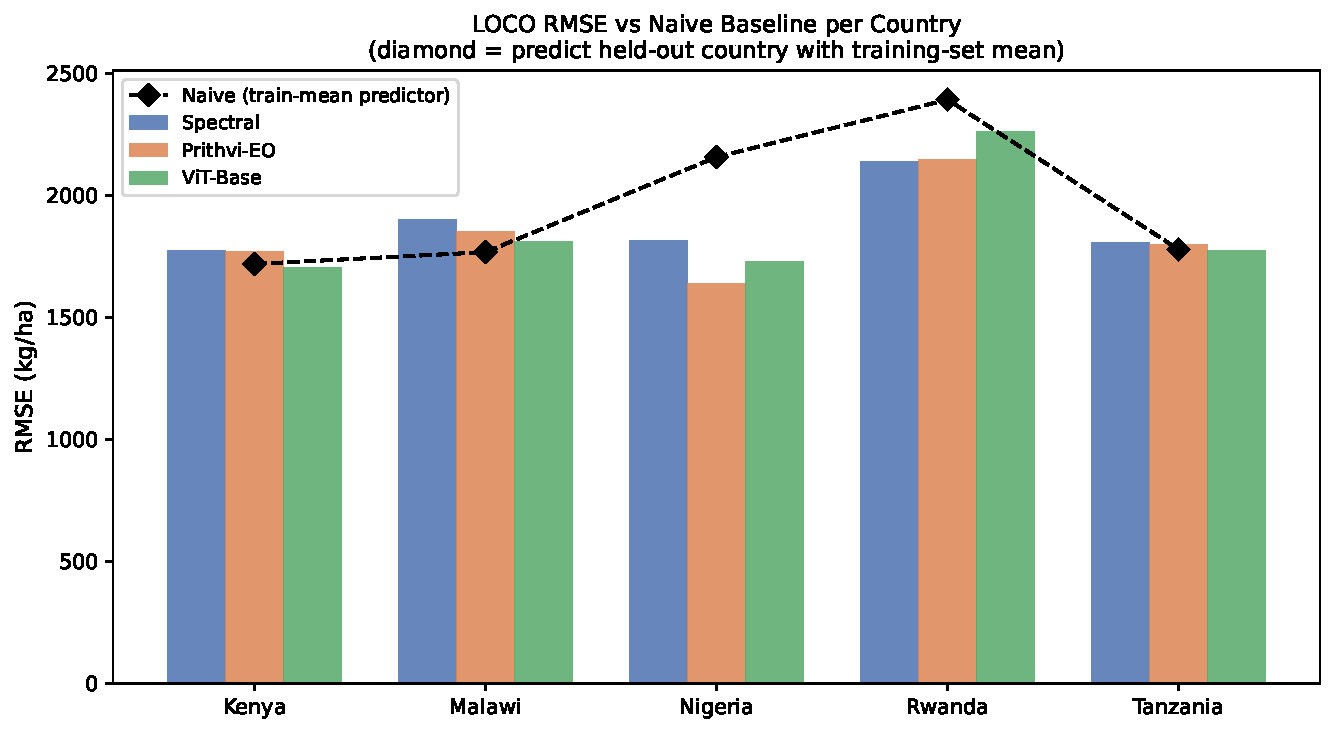
\includegraphics[width=\columnwidth]{../figures/fig5_naive_baseline.pdf}
  \caption{Per-country RMSE for the best model per feature set (bars) vs.\
           the naive country-mean baseline (diamond, dashed line).
           Learned models beat the naive baseline on RMSE, but all remain
           below zero R$^2$.}
  \label{fig:naive}
\end{figure}

Table~\ref{tab:naive} confirms that the naive country-mean predictor
also achieves universally negative R$^2$ under LOCO.
The naive RMSE (1{,}719--2{,}392 kg/ha) exceeds the best-model RMSE
for all countries, indicating that learned representations do provide
some signal beyond the simplest possible predictor.
However, both learned models and the naive baseline lie below zero R$^2$,
confirming that predicting held-out countries from other-country data
is a fundamentally difficult task regardless of model sophistication.

\begin{table}[!t]
  \centering
  \caption{Naive country-mean baseline under LOCO.}
  \label{tab:naive}
  \begin{tabular}{lrrrr}
    \toprule
    Country   & $n_{\text{test}}$ & Naive RMSE (kg/ha) & Naive R$^2$ \\
    \midrule
    Kenya     & 1{,}396           & 1{,}719            & $-0.167$   \\
    Malawi    & 1{,}552           & 1{,}768            & $-0.676$   \\
    Nigeria   & 955               & 2{,}157            & $-2.121$   \\
    Rwanda    & 1{,}138           & 2{,}392            & $-0.631$   \\
    Tanzania  & 1{,}363           & 1{,}779            & $-0.137$   \\
    \bottomrule
  \end{tabular}
\end{table}

\subsection{Generalisation Gap}

\begin{figure}[!t]
  \centering
  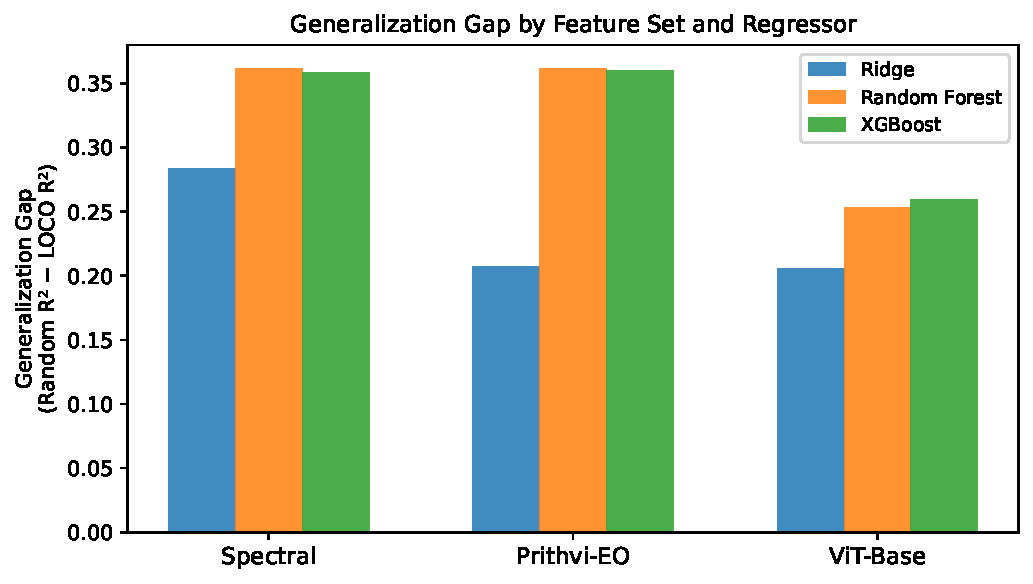
\includegraphics[width=\columnwidth]{../figures/fig4_generalization_gap.pdf}
  \caption{Generalisation gap (random CV R$^2$ minus LOCO R$^2$) per
           feature--regressor combination. Ridge consistently shows smaller
           gaps than tree ensembles despite lower within-country accuracy.}
  \label{fig:gap}
\end{figure}

The generalisation gap — defined as random R$^2$ minus LOCO R$^2$ —
is visualised in Figure~\ref{fig:gap} and ranges from 0.216 (Prithvi-EO / Ridge: $0.180 - (-0.027)$) to
0.384 (Spectral / Ridge: $0.191 - (-0.093)$).
XGBoost, despite being the strongest within-country model, exhibits
generalisation gaps of 0.359 (spectral), 0.360 (Prithvi-EO),
and 0.259 (ViT-Base), demonstrating that higher within-country accuracy
does not imply better cross-country transfer.
Ridge consistently exhibits smaller generalisation gaps than tree
ensembles, suggesting that simpler models are more robust to
distribution shift.

\subsection{Per-Country Analysis}

\begin{figure}[!t]
  \centering
  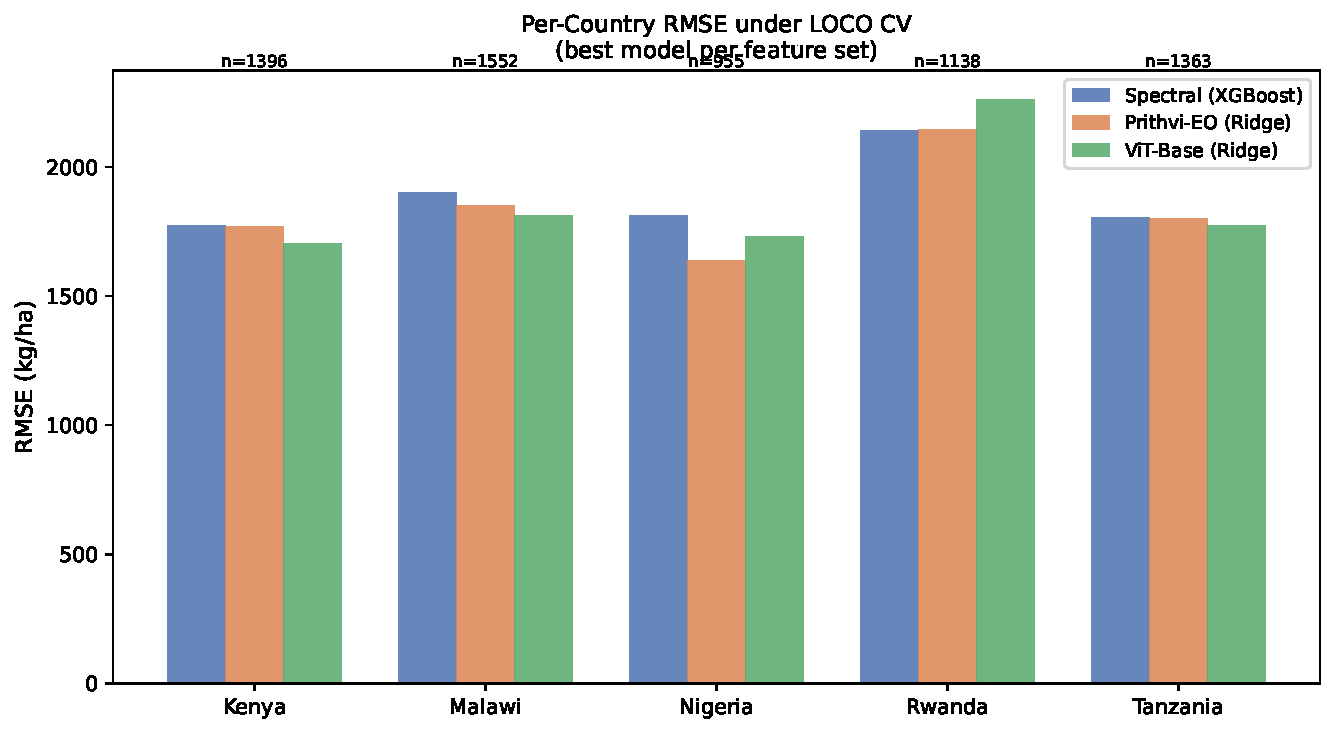
\includegraphics[width=\columnwidth]{../figures/fig3_loco_country_rmse.pdf}
  \caption{Per-country LOCO RMSE (kg/ha) for all nine conditions, with
           test-set sample sizes annotated. Rwanda and Nigeria are
           consistently the most difficult held-out countries.}
  \label{fig:country_rmse}
\end{figure}

\begin{figure*}[!t]
  \centering
  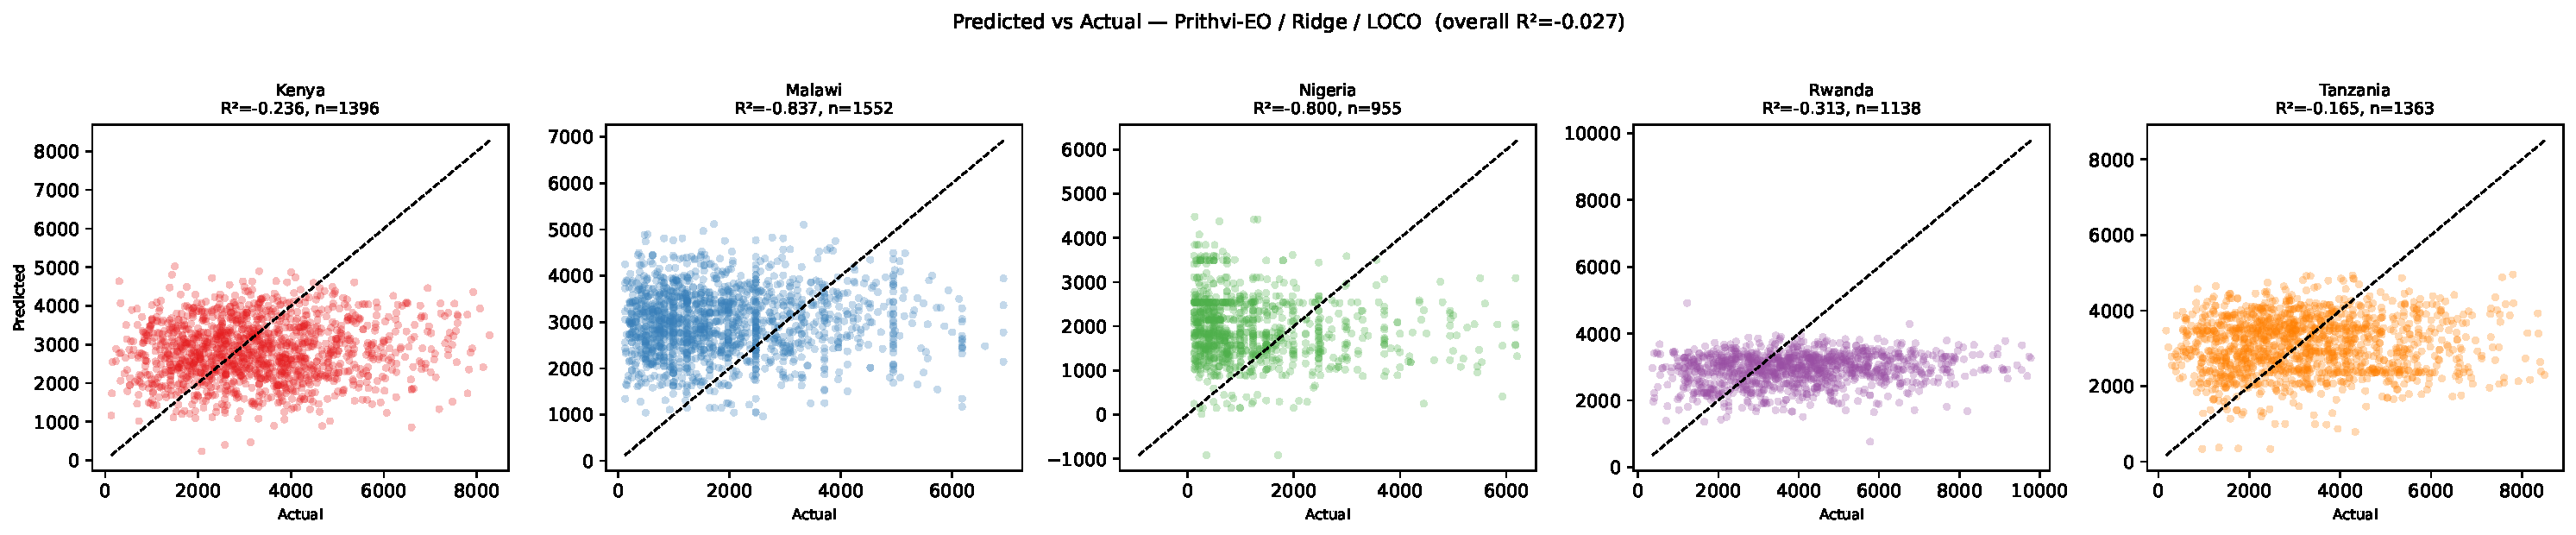
\includegraphics[width=\textwidth]{../figures/fig6_pred_vs_actual.pdf}
  \caption{Predicted vs.\ actual yield scatter under LOCO for the
           Prithvi-EO / Ridge condition (one panel per held-out country).
           The 1:1 line is shown dashed. Systematic under- and
           over-prediction reflects country-level yield distribution shift.}
  \label{fig:scatter}
\end{figure*}

Figure~\ref{fig:country_rmse} shows per-country LOCO RMSE across all conditions
and Figure~\ref{fig:scatter} plots predicted vs.\ actual yield for the Prithvi-EO / Ridge condition.
Rwanda is the hardest held-out country across all conditions
(RMSE $>$ 2{,}100 kg/ha), consistent with its unusually high
mean yield (3{,}993 kg/ha) relative to training-set means.
Nigeria similarly shows the largest naive-baseline deficit
(naive R$^2 = -2.121$), plausibly explained by the use of
admin-centroid proxy observations.
Kenya and Tanzania are easiest to predict (lowest RMSE under LOCO),
likely because their yield ranges overlap more substantially with
the pooled training distribution.

% -------------------------------------------------------------------------
\section{Discussion}
\label{sec:discussion}

\subsection{Why Foundation Models Do Not Close the Gap}

The core finding — that Prithvi-EO embeddings are not meaningfully
superior to spectral features under LOCO — warrants careful interpretation.
We used \emph{frozen} embeddings without task-specific fine-tuning.
Prithvi-EO was pre-trained on six-channel multi-temporal HLS composites
with a reconstruction objective; its CLS token may not encode
agronomically discriminative features unless fine-tuned toward yield.
Moreover, the model was pre-trained predominantly on North American
imagery; domain adaptation to African agroecological conditions was
not performed.
These factors likely prevent the model from providing
representations that transfer across the distinct smallholder systems
of Kenya, Rwanda, Nigeria, Malawi, and Tanzania.

A secondary interpretation is that the problem is irreducibly one of
label shift rather than covariate shift.
Country mean yields span from 1{,}256 kg/ha (Nigeria) to 3{,}993 kg/ha (Rwanda),
a factor of 3.2$\times$.
No feature representation can recover accurate yield magnitudes for
a held-out country if the training-set yield distribution covers a
fundamentally different range.
Addressing label shift requires either normalisation of yield to
country-level benchmarks or richer auxiliary data on soil fertility,
management practices, and input use — information not encoded in
satellite imagery alone.

\subsection{Implications for Benchmarking}

Our results demonstrate concretely that within-country random CV
inflates performance by 0.22--0.38 R$^2$ units relative to LOCO.
Practitioners and reviewers should treat any yield prediction accuracy
figures reported under random within-country CV with commensurate
scepticism when the intended application is cross-country or
cross-region deployment.
LOCO, or at minimum a spatial block CV scheme that prevents
geographic leakage, should be the default evaluation protocol
for operational yield prediction.

\subsection{Limitations}
\label{sec:limits}

Several limitations constrain the scope of our conclusions:

\begin{enumerate}
  \item \textbf{Frozen embeddings only.} Fine-tuning Prithvi-EO on African maize
        data may recover generalisation that frozen inference cannot.
        This remains an important open experiment.
  \item \textbf{Single-timestamp composites.} Prithvi-EO was designed for
        multi-temporal input; using a single growing-season composite
        discards phenological information the model was trained to exploit.
  \item \textbf{Nigeria label quality.} Admin-centroid proxy labels for Nigeria
        introduce spatial mismatch error relative to GPS-tagged fields.
  \item \textbf{Five-country sample.} LOCO over five countries produces five
        test folds; small differences in R$^2$ between feature sets
        ($<0.04$) are not statistically testable at this sample size.
  \item \textbf{No domain adaptation.} Techniques such as domain-adversarial
        training, country-level normalisation, or meta-learning were not
        evaluated and may substantially improve cross-country transfer.
\end{enumerate}

% -------------------------------------------------------------------------
\section{Conclusion}
\label{sec:conclusion}

We evaluated 18 combinations of feature representation, regression algorithm,
and cross-validation scheme for smallholder maize yield prediction across
five sub-Saharan African countries.
Within-country performance is moderate (R$^2$ up to 0.30) but
cross-country generalisation is uniformly poor (all LOCO R$^2 < 0$).
Frozen Prithvi-EO embeddings provide no meaningful advantage over
10-band Sentinel-2 spectral features, implying that geospatial
domain-specific pre-training alone — without fine-tuning or
domain adaptation — is insufficient to overcome country-level
yield distribution shift.
Our work establishes a reproducible LOCO benchmark against which
future domain adaptation and meta-learning approaches for
African crop yield prediction should be compared.

% -------------------------------------------------------------------------
\section*{Data and Code Availability}

The GROW-Africa yield labels are publicly available at
\href{https://doi.org/10.5281/zenodo.14961637}{doi:10.5281/zenodo.14961637}.
All preprocessing, embedding extraction, model training, and figure
generation code is available at
\url{https://github.com/yaw-adjei/yield-africa}.
Processed results (\texttt{results\_all.csv},
\texttt{results\_loco\_country.csv}) and paper figures are included in the
repository.

% -------------------------------------------------------------------------
\section*{Acknowledgements}

The author thanks the GROW-Africa consortium for curating and releasing the
smallholder yield dataset, and IBM Research and NASA for releasing the
Prithvi-EO-1.0-100M model weights under an open licence.
Sentinel-2 imagery was accessed free of charge through the Google Earth Engine
research programme.

% -------------------------------------------------------------------------
\bibliographystyle{IEEEtran}
\bibliography{references}

\end{document}
